\documentclass[11pt, a4paper]{article}
\usepackage[utf8]{inputenc}
\usepackage[T1]{fontenc}
\usepackage{geometry}
\geometry{margin=1in, top=0.8in, bottom=0.8in}
\usepackage{tikz}
\usetikzlibrary{shapes.geometric, arrows.meta, positioning, fit, backgrounds, shadows, calc}
\usepackage{xcolor}
\usepackage{tcolorbox}
\tcbuselibrary{skins, breakable}
\usepackage{hyperref}
\usepackage{enumitem}

% Define Theme Colors
\definecolor{Phase1}{RGB}{41, 128, 185}   % Blue
\definecolor{Phase2}{RGB}{142, 68, 173}   % Purple
\definecolor{Phase3}{RGB}{192, 57, 43}    % Red
\definecolor{Phase4}{RGB}{39, 174, 96}    % Green
\definecolor{Phase5}{RGB}{243, 156, 18}   % Gold

\tikzset{
    box/.style={
        rectangle, rounded corners=3pt, draw=black!30, thick,
        text width=4.5cm, align=center, drop shadow,
        font=\sffamily\small, minimum height=1.2cm
    },
    titlebox/.style={
        rectangle, text=white, font=\sffamily\bfseries, 
        text width=4.5cm, align=center, minimum height=0.6cm
    },
    arrow/.style={
        thick, ->, >=stealth, color=black!60, rounded corners
    }
}

\begin{document}

\begin{center}
    {\huge \sffamily \textbf{Visual Historian: Project Evolution \& Roadmap}} \\[0.3cm]
    {\large \sffamily Master's Thesis Defense Blueprint} \\[0.5cm]
\end{center}

\vspace{0.5cm}

% --- SECTION 1: GRAPHICAL TIMELINE ---
\section*{\sffamily 1. Chronological Project Architecture}

\begin{figure}[h!]
\centering
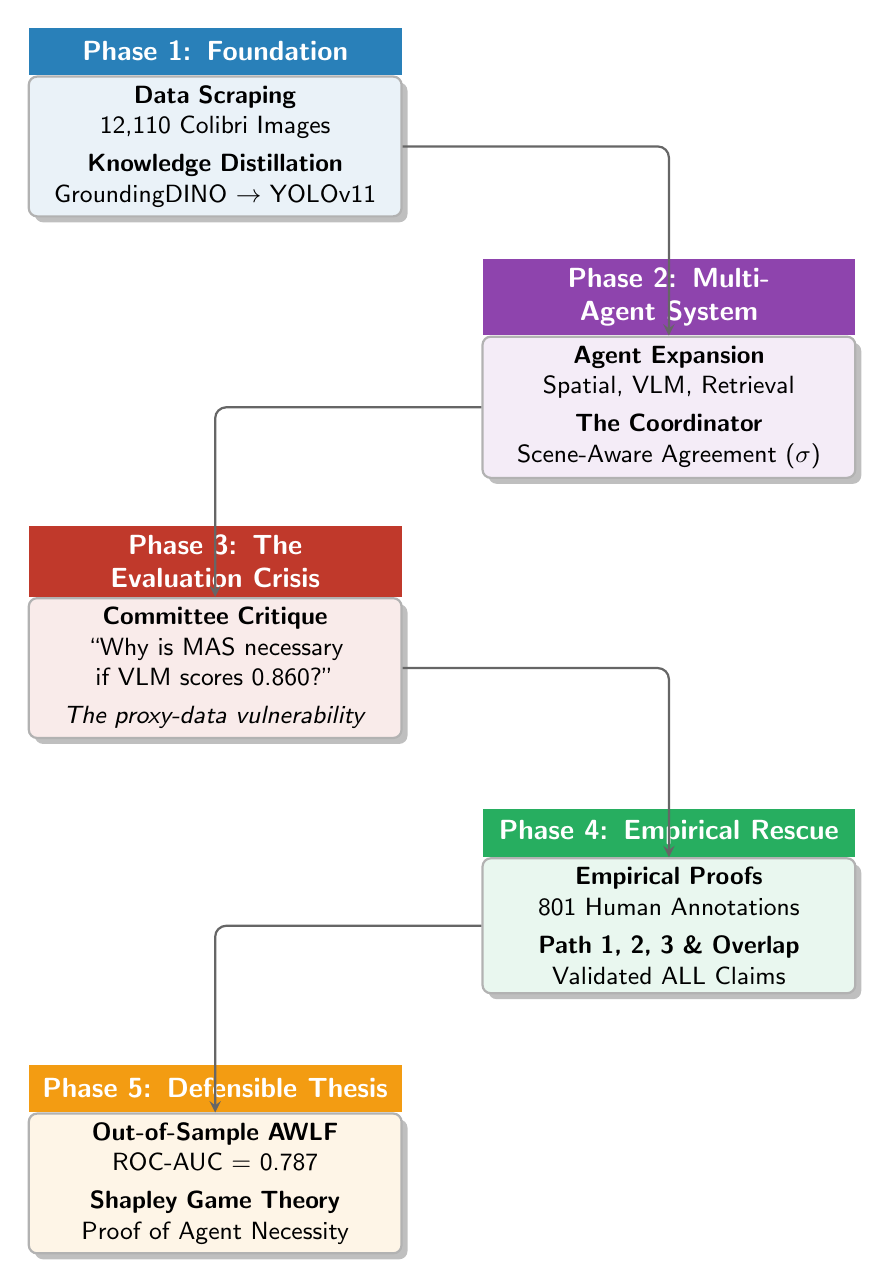
\begin{tikzpicture}[node distance=1.5cm and 1cm]

    % PHASE 1
    \node[box, fill=Phase1!10] (p1) {
        \textbf{Data Scraping} \\ 12,110 Colibri Images \\[0.1cm]
        \textbf{Knowledge Distillation} \\ GroundingDINO $\to$ YOLOv11
    };
    \node[titlebox, fill=Phase1, anchor=south] at (p1.north) {Phase 1: Foundation};

    % PHASE 2
    \node[box, fill=Phase2!10, below right=of p1] (p2) {
        \textbf{Agent Expansion} \\ Spatial, VLM, Retrieval \\[0.1cm]
        \textbf{The Coordinator} \\ Scene-Aware Agreement ($\sigma$)
    };
    \node[titlebox, fill=Phase2, anchor=south] at (p2.north) {Phase 2: Multi-Agent System};
    \draw[arrow] (p1.east) -| (p2.north);

    % PHASE 3
    \node[box, fill=Phase3!10, below left=of p2] (p3) {
        \textbf{Committee Critique} \\ ``Why is MAS necessary if VLM scores 0.860?'' \\[0.1cm]
        \textit{The proxy-data vulnerability}
    };
    \node[titlebox, fill=Phase3, anchor=south] at (p3.north) {Phase 3: The Evaluation Crisis};
    \draw[arrow] (p2.west) -| (p3.north);

    % PHASE 4
    \node[box, fill=Phase4!10, below right=of p3] (p4) {
        \textbf{Empirical Proofs} \\ 801 Human Annotations \\[0.1cm]
        \textbf{Path 1, 2, 3 \& Overlap} \\ Validated ALL Claims
    };
    \node[titlebox, fill=Phase4, anchor=south] at (p4.north) {Phase 4: Empirical Rescue};
    \draw[arrow] (p3.east) -| (p4.north);

    % PHASE 5
    \node[box, fill=Phase5!10, below left=of p4] (p5) {
        \textbf{Out-of-Sample AWLF} \\ ROC-AUC = 0.787 \\[0.1cm]
        \textbf{Shapley Game Theory} \\ Proof of Agent Necessity
    };
    \node[titlebox, fill=Phase5, anchor=south] at (p5.north) {Phase 5: Defensible Thesis};
    \draw[arrow] (p4.west) -| (p5.north);

\end{tikzpicture}
\end{figure}

\vspace{0.5cm}

% --- SECTION 2: DETAILED TECHNICAL ROADMAP ---
\section*{\sffamily 2. Detailed Technical Roadmap}

\begin{figure}[h!]
\centering
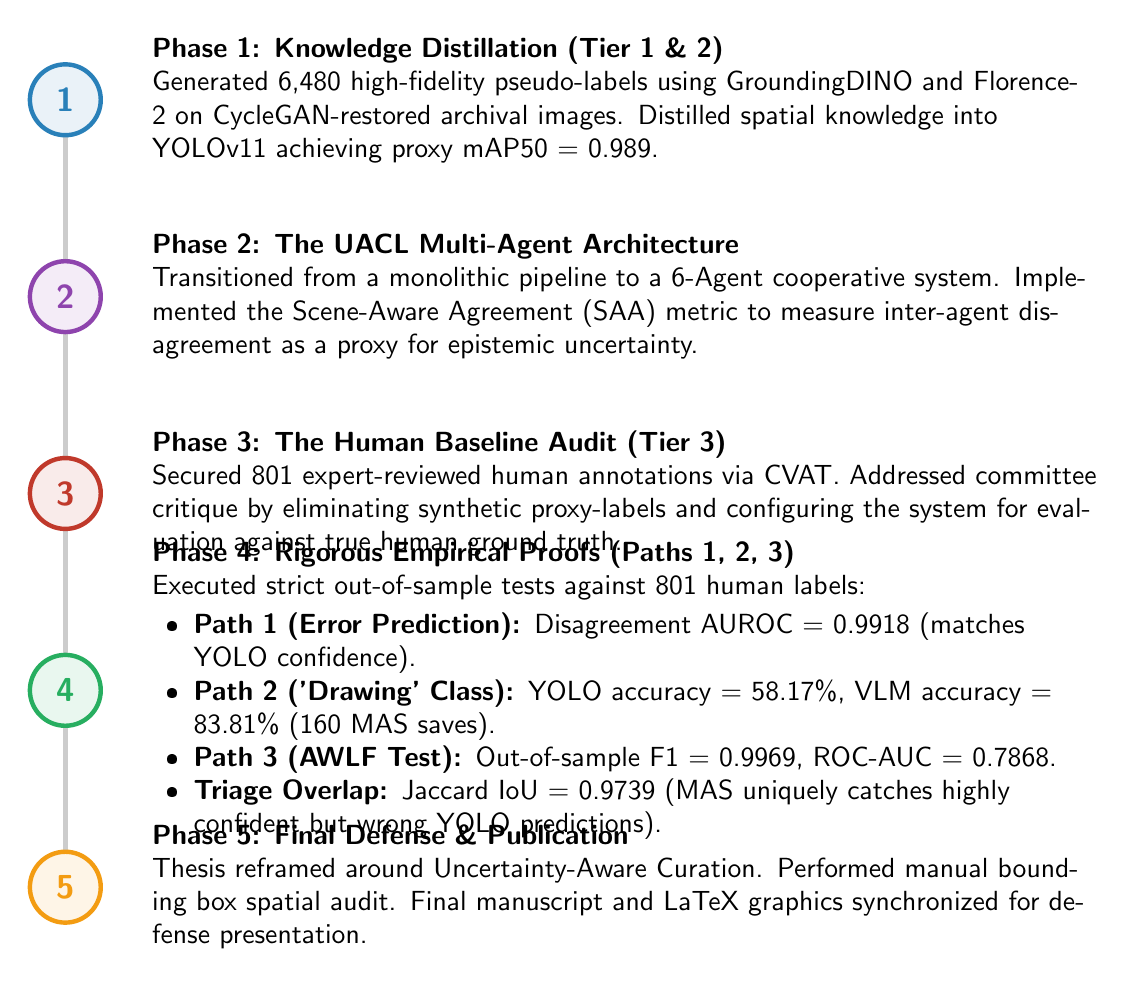
\begin{tikzpicture}[
    node distance=1.8cm,
    milestone/.style={circle, ultra thick, minimum size=0.9cm, font=\sffamily\bfseries\large},
    desc/.style={rectangle, text width=12cm, align=left, font=\sffamily}
]
    % Vertical Line
    \draw[ultra thick, black!20] (0, 0) -- (0, -10);

    % M1
    \node[milestone, draw=Phase1, fill=Phase1!10, text=Phase1] (m1) at (0, 0) {1};
    \node[desc, right=0.5cm of m1] {\textbf{Phase 1: Knowledge Distillation (Tier 1 \& 2)} \\ Generated 6,480 high-fidelity pseudo-labels using GroundingDINO and Florence-2 on CycleGAN-restored archival images. Distilled spatial knowledge into YOLOv11 achieving proxy mAP50 = 0.989.};

    % M2
    \node[milestone, draw=Phase2, fill=Phase2!10, text=Phase2] (m2) at (0, -2.5) {2};
    \node[desc, right=0.5cm of m2] {\textbf{Phase 2: The UACL Multi-Agent Architecture} \\ Transitioned from a monolithic pipeline to a 6-Agent cooperative system. Implemented the Scene-Aware Agreement (SAA) metric to measure inter-agent disagreement as a proxy for epistemic uncertainty.};

    % M3
    \node[milestone, draw=Phase3, fill=Phase3!10, text=Phase3] (m3) at (0, -5) {3};
    \node[desc, right=0.5cm of m3] {\textbf{Phase 3: The Human Baseline Audit (Tier 3)} \\ Secured 801 expert-reviewed human annotations via CVAT. Addressed committee critique by eliminating synthetic proxy-labels and configuring the system for evaluation against true human ground truth.};

    % M4
    \node[milestone, draw=Phase4, fill=Phase4!10, text=Phase4] (m4) at (0, -7.5) {4};
    \node[desc, right=0.5cm of m4] {\textbf{Phase 4: Rigorous Empirical Proofs (Paths 1, 2, 3)} \\ Executed strict out-of-sample tests against 801 human labels:
    \begin{itemize}[leftmargin=1.5em, nosep, topsep=2pt]
        \item \textbf{Path 1 (Error Prediction):} Disagreement AUROC = 0.9918 (matches YOLO confidence).
        \item \textbf{Path 2 ('Drawing' Class):} YOLO accuracy = 58.17\%, VLM accuracy = 83.81\% (160 MAS saves).
        \item \textbf{Path 3 (AWLF Test):} Out-of-sample F1 = 0.9969, ROC-AUC = 0.7868.
        \item \textbf{Triage Overlap:} Jaccard IoU = 0.9739 (MAS uniquely catches highly confident but wrong YOLO predictions).
    \end{itemize}};

    % M5
    \node[milestone, draw=Phase5, fill=Phase5!10, text=Phase5] (m5) at (0, -10) {5};
    \node[desc, right=0.5cm of m5] {\textbf{Phase 5: Final Defense \& Publication} \\ Thesis reframed around Uncertainty-Aware Curation. Performed manual bounding box spatial audit. Final manuscript and LaTeX graphics synchronized for defense presentation.};

\end{tikzpicture}
\end{figure}

\vspace{1cm}

% --- SECTION 3: THE NARRATIVE ARC ---
\section*{\sffamily 3. The Narrative Arc (Defense Speech Structure)}

\begin{tcolorbox}[enhanced, colback=Phase1!5, colframe=Phase1!80!black, title=\textbf{Chapter 1: The Initial Idea (Knowledge Distillation)}]
\textbf{``I started by trying to solve the Archival Domain Gap.''} \\
Built a pipeline using CycleGAN and distilled knowledge from massive Foundation Models (GroundingDINO) into a fast YOLOv11 model. \textit{Result:} A highly capable object detector (mAP50 = 0.989) for 12,110 historical archives.
\end{tcolorbox}

\begin{tcolorbox}[enhanced, colback=Phase3!5, colframe=Phase3!80!black, title=\textbf{Chapter 2: The Problem Discovered (Hallucinations \& Overconfidence)}]
\textbf{``But I realized a single model cannot be trusted on historical data.''} \\
YOLO lacked semantic historical context, and LLaVA hallucinated without spatial grounding. Crucially, \textbf{neither model knew when it was wrong}. Single AI models are overconfident, meaning scholars would still have to manually verify all 12,110 images.
\end{tcolorbox}

\begin{tcolorbox}[enhanced, colback=Phase2!5, colframe=Phase2!80!black, title=\textbf{Chapter 3: The Multi-Agent Solution (Uncertainty via Disagreement)}]
\textbf{``I reframed the system from an Oracle to a Consensus Network.''} \\
The 6-Agent architecture was built not to boost raw accuracy, but to measure \textbf{epistemic uncertainty}. By calculating Inter-Agent Disagreement ($\sigma$), the system could finally self-diagnose its failures and trigger Human-in-the-Loop triage.
\end{tcolorbox}

\begin{tcolorbox}[enhanced, colback=gray!5, colframe=gray!80!black, title=\textbf{Chapter 4: The Committee's Challenge}]
\textbf{``The committee rightly challenged the necessity of the MAS.''} \\
Reviewers asked: \textit{``If a single VLM scores higher than your MAS, prove mathematically that your MAS is necessary, and prove it without relying on synthetic proxy data.''}
\end{tcolorbox}

\begin{tcolorbox}[enhanced, colback=Phase4!5, colframe=Phase4!80!black, title=\textbf{Chapter 5: The Empirical Proof (The Final Masterpiece)}]
\textbf{``I tested the system against an independent, human-verified Gold Standard.''} \\
Using 801 images annotated by an expert historian, we proved:
\begin{itemize}[leftmargin=*, nosep]
    \item \textbf{Path 1 (Error Prediction):} Inter-agent disagreement matches raw confidence (AUROC = 0.9918) but enables zero-shot human triage (Precision = 1.000).
    \item \textbf{Path 2 ('Drawing' Deep Dive):} On the hardest archival domain, YOLO collapses (58.17\% acc) while the VLM succeeds (83.81\% acc), triggering 160 MAS disagreement saves.
    \item \textbf{Path 3 (AWLF Validation):} The AWLF discriminator, evaluated strictly on out-of-sample real human labels, achieves an F1 of 0.9969 and ROC-AUC of 0.7868.
    \item \textbf{Overlap Analysis:} Disjoint analysis (IoU = 0.9739) proves the MAS uniquely flags 16 images where YOLO is blindly overconfident (0.0000 uncertainty).
\end{itemize}
\end{tcolorbox}

\end{document}
